\documentclass[usenames,dvipsnames]{beamer}
\usepackage{../../shared/styles/custom}
\usepackage{../../shared/styles/conventions}




\title{Gradient Descent}
\date{\today}
\author{Nipun Batra}
\institute{IIT Gandhinagar}
\begin{document}
  \maketitle

  \section{Revision}
  \begin{frame}{Contour Plot And Gradients}
	
	$z = f(x,y) = x^{2} + y^{2}$\\
	
	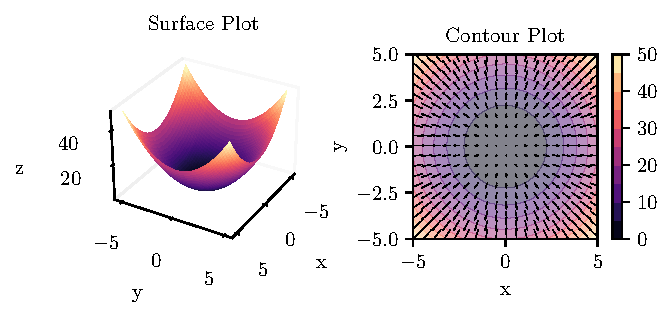
\includegraphics[scale=0.9]{../../maths/assets/mathematical-ml/figures/contour-x_squared_plus_y_squared_quiver-with-gradient.pdf}
	
	


\pause Gradient denotes the direction of steepest ascent or the direction in which there is a maximum increase in f(x,y) \\
\pause $\nabla f(x, y) = \begin{bmatrix}
\frac{\partial f(x, y)}{\partial x}\\
\frac{\partial f(x, y)}{\partial y}
\end{bmatrix} = \begin{bmatrix} 2x\\2y
\end{bmatrix}$



\end{frame}

  \section{Introduction}

  \begin{frame}{Optimization algorithms}
    \begin{itemize}[<+->]
        \item We often want to minimize/maximize a function
        \item We wanted to minimize the cost function:
        \begin{equation}
            f(\vtheta) = (\vy-\mX\vtheta)^T(\vy-\mX\vtheta)
        \end{equation}
        \item Note, here $\vtheta$ is the parameter vector
        \end{itemize}   
  \end{frame}

  \begin{frame}{Optimization algorithms}
    \begin{itemize}[<+->]
        \item In general, we have following components:
        \item Maximize or Minimize a function subject to some constraints
        \item Today, we will focus on unconstrained optimization (no constraints)
        \item We will focus on minimization
        \item Goal: 
        \begin{equation}
            \vtheta^* = \underset{\vtheta}{\argmin}  f(\vtheta)
        \end{equation}
    \end{itemize}
    
  \end{frame}
  
\begin{frame}{Introduction}
    \begin{itemize}[<+->]
    \item Gradient descent is an optimization algorithm
    \item It is used to find the minimum of a function in unconstrained settings
    \item It is an iterative algorithm
    \item It is a first order optimization algorithm
    \item It is a local search algorithm/greedy
    \end{itemize}
\end{frame}



\begin{frame}{Gradient Descent Algorithm} 
    \begin{enumerate}[<+->]
        \item Initialize $\vtheta$ to some random value
        \item Compute the gradient of the cost function at $\vtheta$, $\nabla f(\vtheta)$
        \item For Iteration $i$ ($i = 1,2,\ldots$) or until convergence:
        \begin{itemize}
            \item $\vtheta_{i} \gets   \vtheta_{i-1} - \alpha \nabla f(\vtheta_{i-1})$
        \end{itemize}
    \end{enumerate}
    
\end{frame}
    

  
\section{Taylor's Series}
\begin{frame}{Taylor's Series}
    \begin{itemize}[<+->]
        \item Taylor's series is a way to approximate a function $f(x)$ around a point $x_0$ using a polynomial
        \item The polynomial is given by
        \begin{equation}
            f(x) = f(x_0) + \frac{f'(x_0)}{1!}(x-x_0) + \frac{f''(x_0)}{2!}(x-x_0)^2 + \ldots
        \end{equation}
        \item The vector form of the above equation is given by:
        \begin{equation}
            f(\vx) = f(\vx_0) + \nabla f(\vx_0)^T(\vx-\vx_0) + \frac{1}{2}(\vx-\vx_0)^T\nabla^2 f(\vx_0)(\vx-\vx_0) + \ldots
        \end{equation}
        \item where $\nabla^2 f(\vx_0)$ is the Hessian matrix and $\nabla f(\vx_0)$ is the gradient vector
    \end{itemize}
\end{frame}

    \begin{frame}{Taylor's Series}
        \begin{itemize}[<+->]
            \item Let us consider $f(x) = \cos(x)$ and $x_0 = 0$
            \item Then, we have:
            \item $f(x_0) = \cos(0) = 1$
            \item $f'(x_0) = -\sin(0) = 0$
            \item $f''(x_0) = -\cos(0) = -1$
            \item We can write the second order Taylor's series as:
            \item $f(x) = 1 + 0(x-0) + \frac{-1}{2!}(x-0)^2 = 1 - \frac{x^2}{2}$
        \end{itemize}
        
    \end{frame}

    
    \begin{frame}{Taylor's series}
        \begin{itemize}[<+->]
            \item Let us consider another example: $f(x) = x^2 + 2$ and $x_0 = 2$
            \item Question: How does the first order Taylor's series approximation look like?
            \item First order Taylor's series approximation is given by:
            \item $f(x) = f(x_0) + f'(x_0)(x-x_0) = 6 + 4(x-2) = 4x - 2$
        \end{itemize}
        
    \end{frame}



  \begin{frame}{Taylor's Series (Alternative form)}
    \begin{itemize}[<+->]
    \item We have:
        \begin{equation}
            f(x) = f(x_0) + \frac{f'(x_0)}{1!}(x-x_0) + \frac{f''(x_0)}{2!}(x-x_0)^2 + \ldots
        \end{equation}
    \item Let us consider $x = x_0 + \Delta x$ where $\Delta x$ is a small quantity
    \item Then, we have:
    \begin{equation}
        f(x_0 + \Delta x) = f(x_0) + \frac{f'(x_0)}{1!}\Delta x + \frac{f''(x_0)}{2!}\Delta x^2 + \ldots
    \end{equation} 
    \item Let us assume $\Delta x$ is small enough such that $\Delta x^2$ and higher order terms can be ignored
    \item Then, we have:
    $f(x_0 + \Delta x) \approx f(x_0) + \frac{f'(x_0)}{1!}\Delta x$
    \end{itemize}


	

	
  \end{frame}

  \begin{frame}{Taylor's Series  to Gradient Descent}
    \begin{itemize}[<+->]
    \item Then, we have:
    $f(x_0 + \Delta x) \approx f(x_0) + \frac{f'(x_0)}{1!}\Delta x$
    \item Or, in vector form:
    $f(\vx_0 + \Delta \vx) \approx f(\vx_0) + \nabla f(\vx_0)^T\Delta \vx$
    \item Goal: Find $\Delta \vx$ such that $f(\vx_0 + \Delta \vx)$ is minimized
    \item This is equivalent to minimizing $f(\vx_0) + \nabla f(\vx_0)^T\Delta \vx$
    \item This happens when vectors $\nabla f(\vx_0)$ and $\Delta \vx$ are at phase angle of $180^{\circ}$
    \item This happens when $\Delta \vx = -\alpha \nabla f(\vx_0)$ where $\alpha$ is a scalar
    \item This is the gradient descent algorithm: $\vx_1 = \vx_0 - \alpha \nabla f(\vx_0)$
\end{itemize}
  \end{frame}

  \begin{frame}{Effect of learning rate}
    Low learning rate $\alpha=0.01$ : Converges slowly
    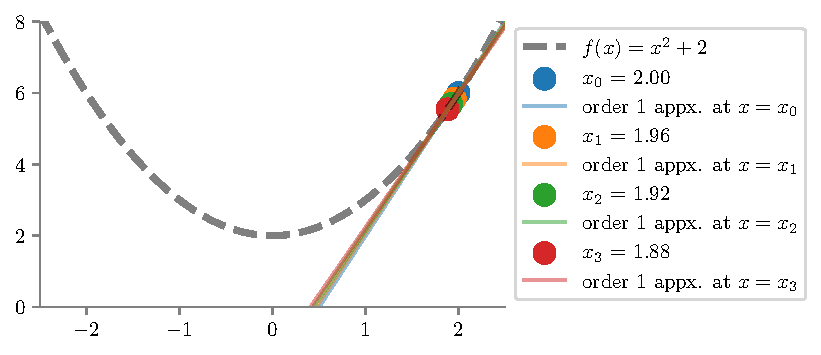
\includegraphics[scale=0.8]{../../maths/assets/mathematical-ml/figures/gd-lr-0.01.pdf}
  \end{frame}

  \begin{frame}{Effect of learning rate}
    High learning rate $\alpha=0.8$: Converges quickly, but might overshoot
    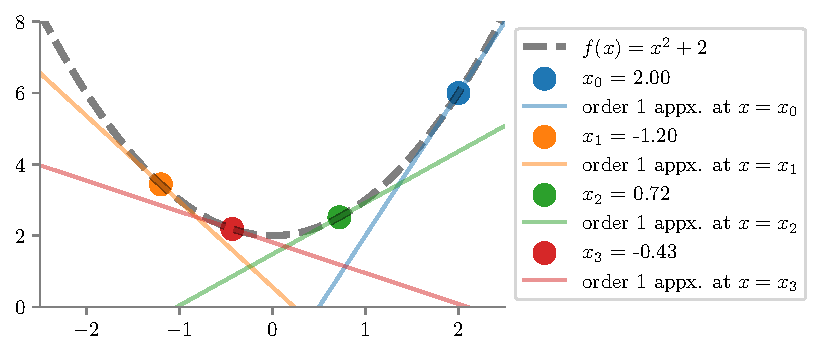
\includegraphics[scale=0.8]{../../maths/assets/mathematical-ml/figures/gd-lr-0.8.pdf}
  \end{frame}

    \begin{frame}{Effect of learning rate}
        Very high learning rate $\alpha=1.01$: Diverges
        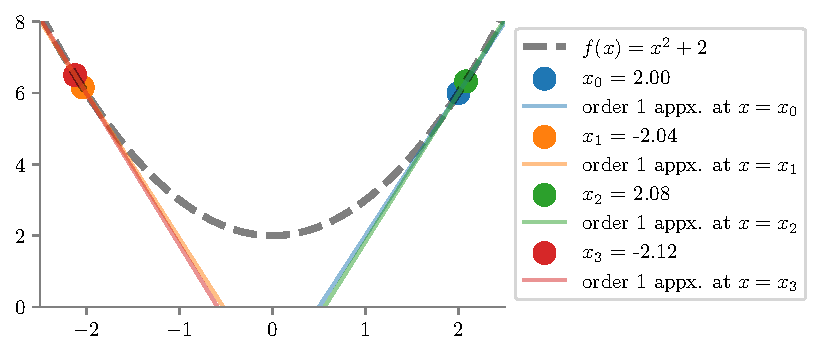
\includegraphics[scale=0.8]{../../maths/assets/mathematical-ml/figures/gd-lr-1.01.pdf}
    \end{frame}


    \begin{frame}{Effect of learning rate}
        Appropriate learning rate $\alpha=0.1$
        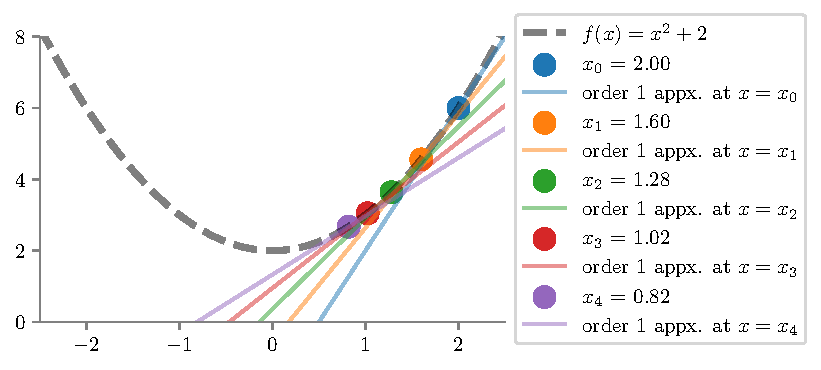
\includegraphics[scale=0.8]{../../maths/assets/mathematical-ml/figures/gd-lr-0.1.pdf}
      \end{frame}

  \section{Gradient Descent for linear regression}
  \begin{frame}{Some commonly confused terms}

    \begin{itemize}[<+->]
        \item \textbf{Loss function} is usually a function defined on a data point, prediction and label, and measures the penalty. 
        \item square loss \(l\left(f\left(x_{i} ; \vtheta\right), y_{i}\right)=\left(f\left(x_{i} ; \vtheta\right)-y_{i}\right)^{2},\) used in linear regression
        \item \textbf{Cost function} is usually more general. It might be a sum of loss functions over your training set plus some model complexity penalty (regularization). For example:
        \item Mean Squared Error \(\MSE(\vtheta)=\frac{1}{n} \sum_{i=1}^{n}\left(f\left(x_{i} ; \vtheta\right)-y_{i}\right)^{2}\)
        \item \textbf{Objective function} is the most general term for any function that you optimize during training.
    \end{itemize}
    
    \end{frame}

    \begin{frame}{Gradient Descent : Example}
        Learn $y = \theta_0 + \theta_1 x$ on following dataset, using gradient descent where initially $(\theta_0, \theta_1) = (4,0)$ and step-size, $\alpha = 0.1$, for 2 iterations. 
        \begin{table}[]
            \centering
            \label{tab:my-table}
            \begin{tabular}{|c|c|}
                \hline
                \textbf{x} & \textbf{y} \\ \hline
                1 & 1 \\ \hline
                2 & 2 \\ \hline
                3 & 3 \\ \hline
            \end{tabular}
        \end{table}
        \end{frame}
        
        

    \begin{frame}{Gradient Descent : Example}
        Our predictor, $\hat{y} = \theta_0 + \theta_1x$\\
        \vspace{1cm}
        Error for $i^{th}$ datapoint, $\epsilon_i = y_i - \hat{y_i}$\\
        $\epsilon_1 = 1 - \theta_0 - \theta_1$ \\
        $\epsilon_2 = 2 - \theta_0 - 2\theta_1$ \\
        $\epsilon_3 = 3 - \theta_0 - 3\theta_1$ \\
        
        \vspace{1cm}
        MSE = $\frac{\epsilon_1^2 + \epsilon_2^2 + \epsilon_3^2}{3}$ = $\frac{14 + 3\theta_0^2 + 14\theta_1^2 -12\theta_0 - 28\theta_1 + 12\theta_0\theta_1}{3}$\\
        \end{frame}
        
            \begin{frame}{Difference between SSE and MSE}
        
        
        
        \begin{equation*}
        \sum \epsilon_{i}^{2} \textit{ increases as the number of examples increase}
        \end{equation*}
        
        So, we use MSE
        
        \begin{equation*}
        \textit{MSE} = \frac{1}{n} \sum \epsilon_{i}^{2}
        \end{equation*}
        
        Here $n$ denotes the number of samples
        
        
        
        \end{frame}

        \begin{frame}{Gradient Descent : Example}
            $\frac{\partial \MSE}{\partial \theta_0} = \frac{2\sum_{i=1}^n \left( y_i - \theta_0 -\theta_1x_i \right)\left(-1\right)}{n} = \frac{2\sum_{i=1}^n \epsilon_i\left(-1\right)}{n}$  
            
            \vspace{2cm}
            $\frac{\partial \MSE}{\partial \theta_1} = \frac{2\sum_{i=1}^n \left( y_i - \theta_0 -\theta_1x_i \right)\left(-x_i\right)}{n} = \frac{2\sum_{i=1}^n \epsilon_i\left(-x_i\right)}{n}$ 
            \end{frame}
            
            \begin{frame}{Gradient Descent : Example}
            \textbf{Iteration 1}\\
            \vspace{0.5cm}
            $\theta_0 = \theta_0 - \alpha\frac{\partial MSE}{\partial \theta_0}$\\ 
            \vspace{0.5cm}
            \only<2->{
            $\theta_0 = 4 - 0.2\frac{\left( (1 - (4 + 0))(-1) + (2 - (4 + 0))(-1) +  (3 - (4 + 0))(-1)  \right)}{3}$\\
            
            \vspace{0.5cm}
            $\theta_0 = 3.6$
            \vspace{0.5cm}
            }
            
            $\theta_1 = \theta_1 - \alpha\frac{\partial MSE}{\partial \theta_1}$\\ 
            \vspace{0.5cm}
            \only<3->{
            $\theta_1	 = 0 - 0.2\frac{\left( (1 - (4 + 0))(-1) + (2 - (4 + 0))(-2) +  (3 - (4 + 0))(-3)  \right)}{3} $\\
            \vspace{0.5cm}
            $\theta_1 = -0.67$
            }
            \end{frame}

            \begin{frame}{Gradient Descent : Example}
                \textbf{Iteration 2}\\
                \vspace{0.5cm}
                $\theta_0 = \theta_0 - \alpha\frac{\partial MSE}{\partial \theta_0}$\\ 
                \vspace{0.5cm}
                \only<2->{
                $\theta_0 = 3.6 - 0.2\frac{\left( (1 - (3.6  - 0.67))(-1) + (2 - (3.6  - 0.67\times 2))(-1) +  (3 - (3.6  - 0.67\times3))(-1)  \right)}{3}$\\ 
                \vspace{0.5cm}
                $\theta_0 = 3.54$\\
                }
                
                \vspace{0.5cm}
                
                $\theta_1 = \theta_1 - \alpha\frac{\partial MSE}{\partial \theta_1}$\\ 
                \vspace{0.5cm}
                \only<3->{
                $\theta_0 = 3.6 - 0.2\frac{\left( (1 - (3.6  - 0.67))(-1) + (2 - (3.6  - 0.67\times 2))(-2) +  (3 - (3.6  - 0.67\times3))(-3)  \right)}{3}$\\ 
                \vspace{0.5cm}
                $\theta_0 = -0.55$\\
                }
                
                \end{frame}
                
                    \foreach \i in {0,2,...,40}{
                        \begin{frame}{Gradient Descent : Example (Iteraion \i)}
                            \begin{figure}
                                \includegraphics[scale=0.7]{../../maths/assets/mathematical-ml/figures/gradient-descent-\i.pdf}
                            \end{figure}
                        \end{frame}
                    }

                    \begin{frame}{Iteration vs Epochs for gradient descent}
                        \begin{itemize}[<+->]
                            \item Iteration: Each time you update the parameters of the model
                            \item Epoch: Each time you have seen all the set of examples
                        \end{itemize}
                    \end{frame}
                    
                        \begin{frame}{Gradient Descent (GD)}
                        \begin{itemize}
                            \item Dataset: $\cD = \{(\mX, \vy)\}$ of size $n$
                            \item Initialize $\vtheta$
                            \item For epoch $e$ in $[1, E]$
                            \begin{itemize}
                                \item Predict $\yhat = \text{pred}(\mX, \vtheta)$
                                \item Compute loss: $J(\vtheta) = \text{loss}(\vy, \yhat)$
                                \item Compute gradient: $\nabla J(\vtheta) = \text{grad}(J)(\vtheta)$
                                \item Update: $\vtheta = \vtheta - \alpha \nabla J(\vtheta)$
                            \end{itemize}
                        \end{itemize}
                    \end{frame}
                    
                    \begin{frame}{Stochastic Gradient Descent (SGD)}
                        \begin{itemize}
                            \item Dataset: $\cD = \{(\mX, \vy)\}$ of size $n$
                            \item Initialize $\vtheta$
                            \item For epoch $e$ in $[1, E]$
                            \begin{itemize}
                                \item Shuffle $\cD$
                                \item For $i$ in $[1, n]$
                                \begin{itemize}
                                    \item Predict $\yhat_i = \text{pred}(\vx_i, \vtheta)$
                                    \item Compute loss: $J(\vtheta) = \text{loss}(y_i, \yhat_i)$
                                    \item Compute gradient: $\nabla J(\vtheta) = \text{grad}(J)(\vtheta)$
                                    \item Update: $\vtheta = \vtheta - \alpha \nabla J(\vtheta)$
                                \end{itemize}
                            \end{itemize}
                        \end{itemize}
                    \end{frame}
                    
                    \begin{frame}{Mini-Batch Gradient Descent (MBGD)}
                        \begin{itemize}
                            \item Dataset: $\cD = \{(\mX, \vy)\}$ of size $n$
                            \item Initialize $\vtheta$
                            \item For epoch $e$ in $[1, E]$
                            \begin{itemize}
                                \item Shuffle $\cD$
                                \item $\text{Batches} = \text{make\_batches}(\cD, B)$
                                \item For $b$ in $\text{Batches}$
                                \begin{itemize}
                                    \item $\mX_b, \vy_b = b$
                                    \item Predict $\yhat_b = \text{pred}(\mX_b, \vtheta)$
                                    \item Compute loss: $J(\vtheta) = \text{loss}(\vy_b, \yhat_b)$
                                    \item Compute gradient: $\nabla J(\vtheta) = \text{grad}(J)(\vtheta)$
                                    \item Update: $\vtheta = \vtheta - \alpha \nabla J(\vtheta)$
                                \end{itemize}
                            \end{itemize}
                        \end{itemize}
                    \end{frame}
                        
                        
                    
                        
                    
                        
                        \begin{frame}{Gradient Descent vs SGD}
                    
                        
                        
                        
                        Vanilla Gradient Descent
                        \begin{itemize}[<+->]
                            \item 
                            in Vanilla (Batch) gradient descent: We update params after going through all the data 
                            \item Smooth curve for Iteration vs Cost
                            \item For a single update, it needs to compute the gradient over all the samples. Hence takes more time
                            
                        \end{itemize}
                        
                        \pause Stochastic Gradient Descent
                        \begin{itemize}[<+->]
                            \item In SGD, we update parameters after seeing each each point
                            \item Noisier curve for iteration vs cost 
                            \item  For a single update, it computes the gradient over one example. Hence lesser time
                        \end{itemize}
                        
                        
                    \end{frame}
                    
                    \begin{frame}{Stochastic Gradient Descent : Example}
                        Learn $y = \theta_0 + \theta_1 x$ on following dataset, using SGD where initially $(\theta_0, \theta_1) = (4,0)$ and step-size, $\alpha  = 0.1$, for 1 epoch (3 iterations). 
                        \begin{table}[]
                            \centering
                            \label{tab:my-table}
                            \begin{tabular}{|c|c|}
                                \hline
                                \textbf{x} & \textbf{y} \\ \hline
                                2 & 2 \\ \hline
                                3 & 3 \\ \hline
                                1 & 1 \\ \hline
                            \end{tabular}
                        \end{table}
                        \end{frame}
                        
                        \begin{frame}{Stochastic Gradient Descent : Example}
                        Our predictor, $\hat{y} = \theta_0 + \theta_1x$\\
                        \vspace{1cm}
                        Error for $i^{th}$ datapoint, $e_i = y_i - \hat{y_i}$\\
                        
                        $\epsilon_1 = 2 - \theta_0 - 2\theta_1$ \\
                        $\epsilon_2 = 3 - \theta_0 - 3\theta_1$ \\
                        $\epsilon_3 = 1 - \theta_0 - \theta_1$ \\
                        
                        \vspace{1cm}
                        While using SGD, we compute the MSE using only 1 datapoint per iteration. \\
                        So MSE is $\epsilon_1^2$ for iteration 1 and $\epsilon_2^2$ for iteration 2.
                        \end{frame}

                        \begin{frame}{Stochastic Gradient Descent : Example}
                            Contour plot of the cost functions for the three datapoints
                            \begin{figure}
                                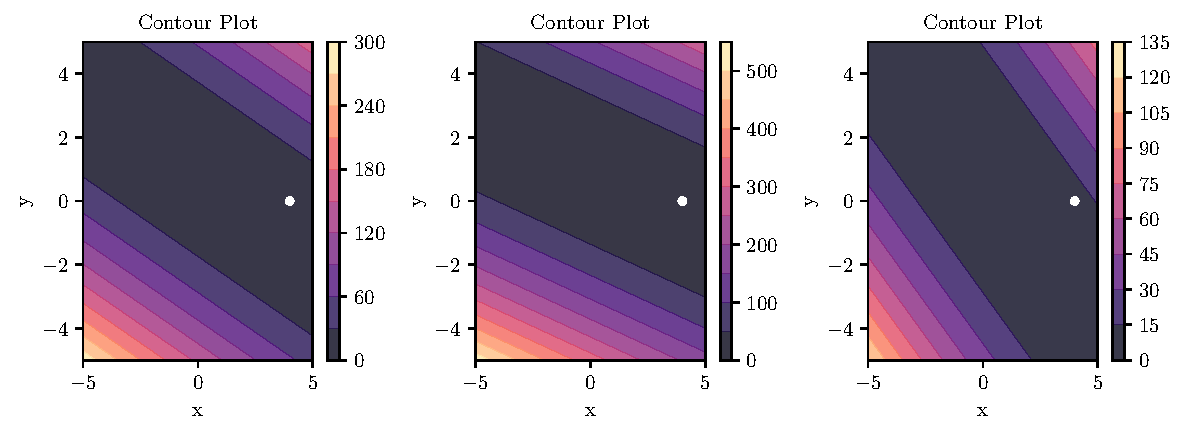
\includegraphics[scale=0.5]{../../maths/assets/mathematical-ml/figures/gradient-descent-3-functions.pdf}
                            \end{figure}
                        \end{frame}
                        
                        
                        \begin{frame}{Stochastic Gradient Descent : Example}
                        \textbf{For Iteration $i$}\\
                        \vspace{1cm}
                        $\frac{\partial MSE}{\partial \theta_0} = 2\left( y_i - \theta_0 -\theta_1x_i \right)\left(-1\right) = 2\epsilon_i\left(-1\right)$ \\
                        \vspace{2cm}
                        $\frac{\partial MSE}{\partial \theta_1} = 2\left( y_i - \theta_0 -\theta_1x_i \right)\left(-x_i\right) = 2\epsilon_i\left(-x_i\right)$ 
                        \end{frame}
                        
                        \begin{frame}{Stochastic Gradient Descent : Example}
                        \textbf{Iteration 1}\\
                        \vspace{0.5cm}
                        $\theta_0 = \theta_0 - \alpha\frac{\partial MSE}{\partial \theta_0}$\\ 
                        \vspace{0.5cm}
                        \only<2->{
                        $\theta_0 = 4 - 0.1 \times 2 \times \left( 2 - (4 + 0) \right)(-1)$\\
                        
                        \vspace{0.5cm}
                        $\theta_0 = 3.6$
                        \vspace{0.5cm}
                        }
                        
                        $\theta_1 = \theta_1 - \alpha\frac{\partial MSE}{\partial \theta_1}$\\ 
                        \vspace{0.5cm}
                        \only<3->{
                        $\theta_1 = 0 - 0.1 \times 2 \times \left( 2 - (4 + 0) \right)(-2)$\\
                        \vspace{0.5cm}
                        $\theta_1 = -0.8$
                        }
                        \end{frame}
                        
                        \begin{frame}{Stochastic Gradient Descent : Example}
                        \textbf{Iteration 2}\\
                        \vspace{0.5cm}
                        $\theta_0 = \theta_0 - \alpha\frac{\partial MSE}{\partial \theta_0}$\\ 
                        \vspace{0.5cm}
                        \only<2->{
                        $\theta_0 = 3.6 - 0.1 \times 2 \times \left( 3 - (3.6 - 0.8 \times 3 )\right)(-1) $\\
                        
                        \vspace{0.5cm}
                        $\theta_0 = 3.96$
                        \vspace{0.5cm}
                        }
                        
                        $\theta_1 = \theta_1 - \alpha\frac{\partial MSE}{\partial \theta_1}$\\ 
                        \vspace{0.5cm}
                        \only<3->{
                        $\theta_0 = -0.8 - 0.1 \times 2 \times \left( 3 - (3.6 - 0.8 \times 3 ) \right)(-3)$\\
                        \vspace{0.5cm}
                        $\theta_1 = 0.28$
                        }
                        \end{frame}
                        
                        \begin{frame}{Stochastic Gradient Descent : Example}
                        \textbf{Iteration 3}\\
                        \vspace{0.5cm}
                        $\theta_0 = \theta_0 - \alpha\frac{\partial MSE}{\partial \theta_0}$\\ 
                        \vspace{0.5cm}
                        \only<2->{
                        $\theta_0 = 3.96 - 0.1 \times 2 \times \left( 1 - (3.96 + 0.28 \times 1 )\right)(-1) $\\
                        
                        \vspace{0.5cm}
                        $\theta_0 = 3.312$
                        \vspace{0.5cm}
                        }
                        
                        $\theta_1 = \theta_1 - \alpha\frac{\partial MSE}{\partial \theta_1}$\\ 
                        \vspace{0.5cm}
                        \only<3->{
                        $\theta_0 = 0.28 - 0.1 \times 2 \times \left( 1 - (3.96 + 0.28 \times 1 )\right)(-1) $\\
                        \vspace{0.5cm}
                        $\theta_1 = -0.368$
                        }
                        \end{frame}
                                       
                        
    \section{Stochastic gradient is an unbiased estimator of the true gradient}


    \begin{frame}{True Gradient}
        Based on Estimation Theory and Machine Learning by Florian Hartmann

        \begin{itemize}[<+->]
            \item Let us say we have a dataset $\mathcal{D}$ containing input output pairs $\{(x_1, y_1), (x_2, y_2), \ldots, (x_N, y_N)\}$
            \item We can define overall loss as:
                $$L(\theta) = \frac{1}{N}\sum_{i=1}^{N}loss(f(x_i, \theta), y_i)$$
            \item loss can be any loss function such as squared loss, cross-entropy loss etc.
            $$loss(f(x_i, \theta), y_i) = (f(x_i, \theta) - y_i)^2$$
        \end{itemize}
    \end{frame}

    \begin{frame}{True Gradient}
        \begin{itemize}[<+->]
            \item The true gradient of the loss function is given by:
            $$
            \begin{aligned}
                \nabla L & =\nabla \frac{1}{n} \sum_{i=1}^n \operatorname{loss}\left(f\left(x_i\right), y_i\right) \\
                & =\frac{1}{n} \sum_{i=1}^n \nabla \operatorname{loss}\left(f\left(x_i\right), y_i\right)
                \end{aligned}
            $$
            \item The above is a consequence of linearity of the gradient operator.
        \end{itemize}
            
        
    \end{frame}

    \begin{frame}{Estimator for the true gradient}
        \begin{itemize}[<+->]
            \item In practice, we do not have access to the true gradient
            \item We can only estimate the true gradient using a subset of the data
            \item For SGD, we use a single example to estimate the true gradient, for mini-batch gradient descent, we use a mini-batch of examples to estimate the true gradient
            \item Let us say we have a sample: (x, y)
            \item The estimated gradient is given by:
            $$\nabla \tilde{L}=\nabla \operatorname{loss}(f(x), y)$$
        \end{itemize}
        
    \end{frame}

    \begin{frame}{Bias of the estimator}
        \begin{itemize}[<+->]
            \item One measure for the quality of an estimator $\tilde{X}$ is its bias or how far off its estimate is on average from the true value $X$ :
            $$
            \operatorname{bias}(X)=\mathbb{E}[\tilde{X}]-X
            $$
           
            \item Using the rules of expectation, we can show that the expected value of the estimated gradient is the true gradient:
            $$
            \begin{aligned}
                \mathbb{E}[\nabla \tilde{L}] & =\sum_{i=1}^n \frac{1}{n} \nabla \operatorname{loss}\left(f\left(x_i\right), y_i\right) \\
                & =\frac{1}{n} \nabla \sum_{i=1}^n \operatorname{loss}\left(f\left(x_i\right), y_i\right) \\
                & =\nabla L
                \end{aligned}
                $$
                \item Thus, the estimated gradient is an unbiased estimator of the true gradient
        \end{itemize}
        
    \end{frame}

    % {
% \setbeamercolor{background canvas}{bg=}
% 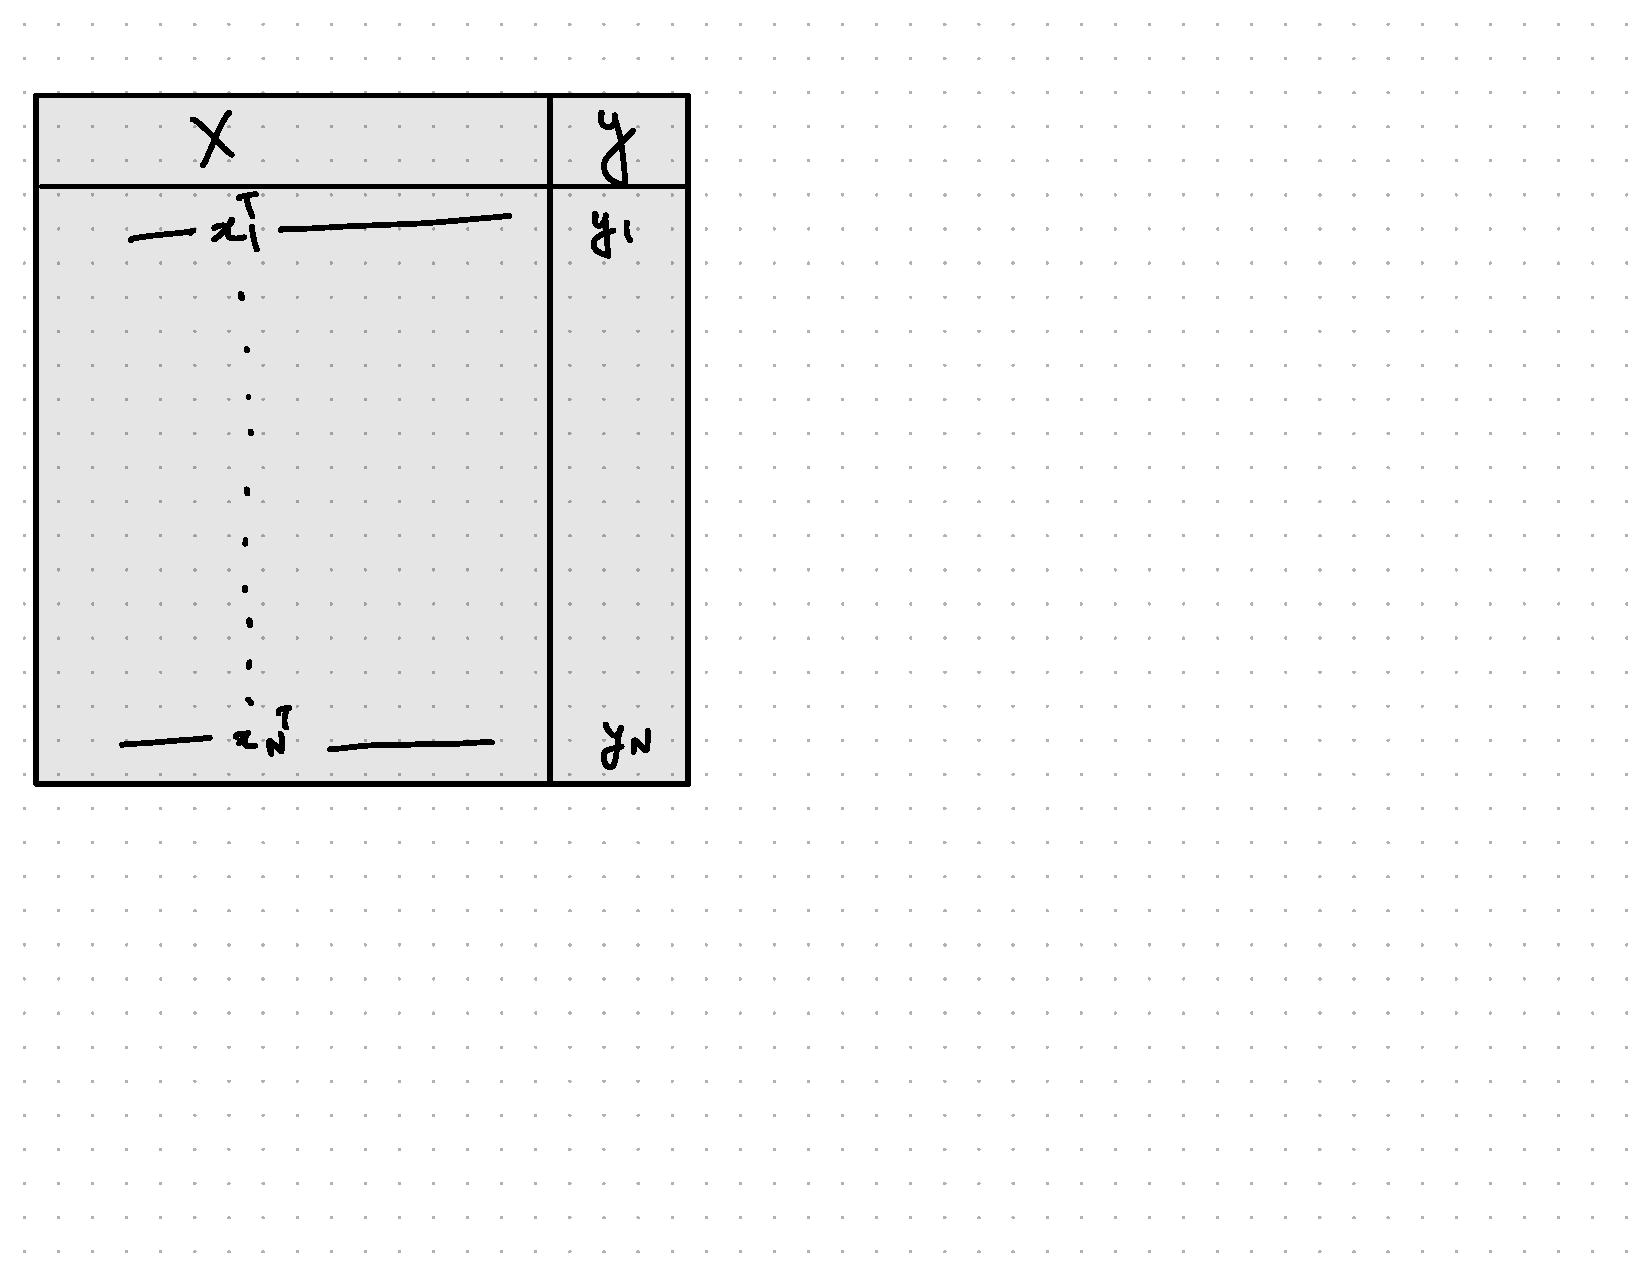
\includepdf[pages=1-]{../assets/SGD.pdf}
% }
                

  \section{Time Complexity: Gradient Descent vs Normal Equation for Linear Regression}
  \begin{frame}{Normal Equation}

	\begin{itemize}[<+->]
		\item Consider $\mX \in \Real^{n \times d}$
		\item $n$ examples and $d$ dimensions
		\item What is the time complexity of solving the normal equation $\hat{\vtheta} = (\mX^T\mX)^{-1}\mX^T\vy$?
	\end{itemize}
	
	

\end{frame}

\begin{frame}{Normal Equation}

\begin{itemize}[<+->]
	\item $\mX$ has dimensions $n \times d$, $\mX^T$ has dimensions $d \times n$
	\item $\mX^T\mX$ is a matrix product of matrices of size: $d \times n$ and $n \times d$, which is $\mathcal{O}(d^{2}n)$
	\item Inversion of $\mX^T\mX$ is an inversion of a $d \times d$ matrix, which is $\mathcal{O}(d^{3})$
	\item $\mX^T\vy$ is a matrix vector product of size $d \times n$ and $n \times 1$, which is $\mathcal{O}(dn)$
	\item $(\mX^T\mX)^{-1}\mX^T\vy$ is a matrix product of a $d \times d$ matrix and $d \times 1$ matrix, which is $\mathcal{O}(d^2)$
	\item Overall complexity: $\mathcal{O}(d^{2}n)$ + $\mathcal{O}(d^{3})$ + $\mathcal{O}(dn)$ + $\mathcal{O}(d^2)$ = $\mathcal{O}(d^{2}n)$ + $\mathcal{O}(d^{3})$
	\item Scales cubic in the number of columns/features of $\mX$
\end{itemize}



\end{frame}


\begin{frame}{Gradient Descent}
Start with random values of $\theta_{0}$ and $\theta_{1}$\\
Till convergence
\begin{itemize}[<+->]
	\item $\theta_{0} = \theta_{0} - \alpha\frac{\partial}{\partial \theta_{0}} (\sum \epsilon_{i}^{2}) $
	\item $\theta_{1} = \theta_{1} - \alpha \frac{\partial}{\partial \theta_{1}} (\sum \epsilon_{i}^{2}) $
	\item Question: Can you write the above for $d$ dimensional data in vectorised form?
	\item	\(\theta_{0}=\theta_{0}-\alpha \frac{\partial}{\partial \theta_{0}}\left(\vy-\mX\vtheta\right)^{\top}\left(\vy-\mX\vtheta\right)\)
	\(\theta_{1}=\theta_{1}-\alpha \frac{\partial}{\partial \theta_{1}}\left(\vy-\mX\vtheta\right)^{\top}\left(\vy-\mX\vtheta\right)\) 
	\\ $\vdots$
	\\	\(\theta_{d}=\theta_{d}-\alpha \frac{\partial}{\partial \theta_{d}}\left(\vy-\mX\vtheta\right)^{\top}\left(\vy-\mX\vtheta\right)\)
	\item \(\vtheta=\vtheta - \alpha \frac{\partial}{\partial \vtheta}\left(\vy-\mX\vtheta\right)^{\top}\left(\vy-\mX\vtheta\right)\) 

\end{itemize}
\end{frame}

\begin{frame}{Gradient Descent}


\(\frac{\partial}{\partial \vtheta}(\vy-\mX \vtheta)^{\top}(\vy-\mX \vtheta)\)
\\ \(=\frac{\partial}{\partial \vtheta}\left(\vy^{\top}-\vtheta^{\top} \mX^{\top}\right)(\vy-\mX \vtheta)\)
\\ \(=\frac{\partial}{\partial \vtheta}\left(\vy^{\top} \vy-\vtheta^{\top} \mX^{\top} \vy-\vy^{\top} \mX \vtheta+\vtheta^{\top} \mX^{\top} \mX \vtheta\right)\)
\\ \(=-2 \mX^{\top} \vy+2 \mX^{\top} \mX \vtheta\)
\\ \(=2 \mX^{\top}(\mX \vtheta-\vy)\)
	

\end{frame}

\begin{frame}{Gradient Descent}


We can write the vectorised update equation as follows, for each iteration

\(\vtheta=\vtheta - \alpha \mX^{\top}(\mX \vtheta-\vy)\) 


\pause For $t$ iterations, what is the computational complexity of our gradient descent solution?

\pause Hint, rewrite the above as: \(\vtheta=\vtheta - \alpha \mX^{\top}\mX \vtheta+ \alpha \mX^{\top}\vy\) 

\pause Complexity of computing $\mX^{\top}\vy$ is $\mathcal{O}(dn)$

\pause Complexity of computing $\alpha \mX^{\top}\vy$ once we have $\mX^{\top}\vy$ is $\mathcal{O}(d)$ since $\mX^{\top}\vy$ has $d$ entries

\pause Complexity of computing $\mX^{\top}\mX$ is $\mathcal{O}(d^2n)$ and then multiplying with $\alpha$ is $\mathcal{O}(d^2)$

\pause All of the above need only be calculated once!



\end{frame}



\begin{frame}{Gradient Descent}
\pause For each of the $t$ iterations, we now need to first multiply $\alpha \mX^{\top}\mX$ with $\vtheta$ which is matrix multiplication of a $d \times d$ matrix with a $d \times 1$, which is $\mathcal{O}(d^2)$ 

\pause The remaining subtraction/addition can be done in $\mathcal{O}(d)$ for each iteration.

\pause What is overall computational complexity?

\pause $\mathcal{O}(td^2)$ + $\mathcal{O}(d^2n) = \mathcal{O}((t+n)d^2)$
\end{frame}

\begin{frame}{Gradient Descent (Alternative)}
\pause If we do not rewrite the expression
\(\vtheta=\vtheta - \alpha \mX^{\top}(\mX \vtheta-\vy)\) 

For each iteration, we have:
\begin{itemize}[<+->]
	\item Computing $\mX\vtheta$ is $\mathcal{O}(nd)$
	\item Computing $\mX\vtheta - \vy$ is $\mathcal{O}(n)$
	\item Computing $\alpha \mX^{\top}$ is $\mathcal{O}(nd)$
	\item Computing $\alpha \mX^{\top}(\mX\vtheta - \vy)$ is $\mathcal{O}(nd)$
	\item Computing \(\vtheta=\vtheta - \alpha \mX^{\top}(\mX \vtheta-\vy)\) is $\mathcal{O}(n)$
\end{itemize}

\pause What is overall computational complexity?

\pause $\mathcal{O}(ndt)$
\end{frame}

 
\end{document}
